\section{Overview and Theoretical Context}
%{\it Assigned to:} {\bf Mayly Sanchez} 

\label{sec:physics-lbnosc-context}

% {\bf [Note: Copied from Section 2.2 of the LBNE Science Document.]}  
The Standard Model of particle physics presents a remarkably accurate
description of the elementary particles and their
interactions. However, its limitations pose deeper questions about
Nature. With the discovery of the Higgs boson at the \dword{cern}, the Standard
Model would be ``complete'' except for the discovery of neutrino
mixing, which indicates neutrinos had a very small but nonzero
mass. In the \dword{sm}, %Standard Model, 
the simple Higgs mechanism is responsible
for both quark and charged lepton masses, quark mixing and
\dword{cpv}. %charge-parity (CP) violation. 
However, the small size of neutrino
masses and their relatively large mixing bears little resemblance to
quark masses and mixing, suggesting that different physics -- and
possibly different mass scales -- in the two sectors may be present,
thus motivating precision study of mixing and \dword{cpv} %CP violation 
in the
lepton sector of the Standard Model. 
%\fixme{thus motivating?}

%\fixme{Wrote a better opening paragraph using text from the Sci. Opp. - MB}

The \dword{dune} plans to pursue a detailed study of neutrino mixing, resolve the
neutrino mass ordering, and search for \dword{cpv} %CP violation 
in the lepton
sector by studying the oscillation patterns of
high-intensity \numu and \anumu %$\nu_\mu$ and $\bar{\nu}_\mu$
beams measured over a long baseline.  Neutrino oscillation arises from
mixing between the flavor 
(\nue, \numu, \nutau) and mass $(\nu_1,\, \nu_2,\, \nu_3)$ eigenstates
of neutrinos.
% corresponding to the weak and gravitational interactions, respectively. 
% This three-flavor-mixing
% scenario can be described by a rotation between the weak-interaction
% eigenstate basis $(\nu_e,\, \nu_\mu,\, \nu_\tau)$ and the basis of
% states of definite mass $(\nu_1,\, \nu_2,\, \nu_3)$.  
In direct correspondence with mixing in the quark sector, the transformation
between basis states is expressed in the form of a complex unitary
matrix, known as the \dword{pmns} matrix: % \textit{PMNS mixing matrix}: 

\begin{equation}
\left(\begin{array}{ccc} \nu_e \\ \nu_\mu \\ \nu_\tau \end{array} \right)= 
\underbrace{
  \left(\begin{array}{ccc}
      U_{e 1} &  U_{e 2} & U_{e 3} \\ 
      U_{\mu1} &  U_{\mu2} & U_{\mu 3} \\ 
      U_{\tau 1} &  U_{\tau 2} & U_{\tau 3} 
    \end{array} \right)
}_{U_{\rm PMNS}} \left(\begin{array}{ccc} \nu_1 \\ \nu_2 \\ \nu_3 \end{array} \right).
\label{eqn:pmns0}
\end{equation}
The \dword{pmns} matrix in full generality depends on just three mixing angles
and a \dword{cp}-violating phase\footnote{In the case of Majorana neutrinos, there are two additional \dword{cp} phases, but they are unobservable in the oscillation processes.}.  The mixing angles and phase are designated
as $(\theta_{12},\, \theta_{23},\, \theta_{13})$ and
\deltacp.
This matrix can be expressed as the product of three
two-flavor mixing matrices as follows~\cite{Schechter:1980gr}, where $c_{\alpha \beta}=\cos \theta_{\alpha \beta}$ and $s_{\alpha
 \beta}=\sin \theta_{\alpha \beta}$:

\begin{equation}
U_{\rm PMNS} = 
  \underbrace{
    \left( \begin{array}{ccc}
        1 & 0 & 0 \\ 
        0 & c_{23} & s_{23} \\ 
        0 & -s_{23} & c_{23}
    \end{array} \right)
  }_{\rm I}
\underbrace{
  \left( \begin{array}{ccc}
        c_{13} & 0  & e^{-i\mdeltacp} s_{13} \\ 
         0 & 1 & 0 \\ 
        -e^{i\mdeltacp} s_{13} & 0 & c_{13}
  \end{array} \right)   
  }_{\rm II}
\underbrace{
 \left( \begin{array}{ccc}
      c_{12} & s_{12} & 0 \\ 
      -s_{12} & c_{12} & 0 \\ 
      0 & 0 & 1
  \end{array} \right)
}_{\rm III}.
\label{eqn:pmns}
\end{equation}

The parameters of the \dword{pmns}
matrix determine the probability amplitudes of the neutrino
oscillation phenomena that arise from mixing.  The frequency of neutrino oscillation 
depends on the difference in the squares of the neutrino
masses, $\Delta m^{2}_{ij} \equiv m^{2}_{i} - m^{2}_{j}$; a set of three
neutrino mass states implies two independent mass-squared differences
(the ``solar'' mass splitting, $\Delta m^{2}_{21}$, and the ``atmospheric'' mass splitting, 
$\Delta m^{2}_{31}$), where $\Delta m^{2}_{31} = \Delta m^{2}_{32} + \Delta m^{2}_{21}$. 
%The numbering of the neutrino mass states is arbitrary; by convention, the numbering is defined such that the solar mass splitting is positive. 
The use of numbers to label the neutrino mass states is arbitrary; by convention, the numbering is defined such that the solar mass splitting is positive, in accordance to the ordering determined from solar matter effects.
This leaves two possibilities for
the ordering of the
mass states, known as the \emph{neutrino mass ordering} or \emph{neutrino mass hierarchy}. An ordering of
$m_1 < m_2 < m_3$ is known as the \emph{normal ordering} since it matches
the mass ordering of the charged leptons in the Standard Model, whereas an ordering of $m_3 < m_1 < m_2$
is referred to as the \emph{inverted ordering}.

The entire complement of neutrino experiments to date has measured
five of the mixing parameters~\cite{Esteban:2018azc,deSalas:2017kay,Capozzi:2017yic}: the three angles $\theta_{12}$,
$\theta_{23}$, and $\theta_{13}$, and the two mass differences
$\Delta m^{2}_{21}$ and $\Delta m^{2}_{31}$. 
%The sign of $\Delta
%m^{2}_{21}$ is fixed by convention, but 
The neutrino mass ordering (i.e., the sign of $\Delta m^{2}_{31}$) is unknown.
The values of $\theta_{12}$ and $\theta_{23}$ are large, while 
$\theta_{13}$ is smaller. The value of \deltacp is not well known, though neutrino oscillation data are beginning to provide some information on its value.
The absolute values of the entries of the \dword{pmns} matrix, which
contains information on the strength of flavor-changing weak decays in
the lepton sector, can be expressed in approximate form as
\begin{equation}
|U_{\rm PMNS}|\sim \left(\begin{array}{ccc} 0.8 & 0.5 & 0.1 \\ 0.5 & 0.6 & 0.7 \\ 0.3 & 0.6 & 0.7\end{array} \right),
\label{eq:pmnsmatrix}
\end{equation}
using values for the mixing angles given in Table~\ref{tab:oscpar_nufit}. 
While the three-flavor-mixing scenario for neutrinos is now well
established, the mixing parameters are not known to the same precision 
as are those in the
corresponding quark sector, and several important quantities, including
the value of \deltacp and the sign of the large mass splitting, are
still undetermined.

The oscillation probability of \numu $\rightarrow$ \nue through matter in a constant density
approximation is,  % Anne 3/9
to first order~\cite{Nunokawa:2007qh}:
%
\begin{eqnarray}
P(\nu_\mu \rightarrow \nu_e) & \simeq & \sin^2 \theta_{23} \sin^2 2 \theta_{13} 
\frac{ \sin^2(\Delta_{31} - aL)}{(\Delta_{31}-aL)^2} \Delta_{31}^2\\ \nonumber
& & + \sin 2 \theta_{23} \sin 2 \theta_{13} \sin 2 \theta_{12} \frac{ \sin(\Delta_{31} - aL)}{(\Delta_{31}-aL)} \Delta_{31} \frac{\sin(aL)}{(aL)} \Delta_{21} \cos (\Delta_{31} + \mdeltacp)\\ \nonumber
& & + \cos^2 \theta_{23} \sin^2 2 \theta_{12} \frac {\sin^2(aL)}{(aL)^2} \Delta_{21}^2, \\ \nonumber
\label{eqn:appprob}
\end{eqnarray}
where $\Delta_{ij} = \Delta m^2_{ij} L/4E_\nu$, $a = G_FN_e/\sqrt{2}$, $G_F$ is the Fermi constant, $N_e$ is the number density of electrons in the Earth, $L$ is the baseline in km, and $E_\nu$ is the neutrino energy in GeV. 
In the equation above, both \deltacp and $a$ 
switch signs in going from the
$\nu_\mu \to \nu_e$ to the $\bar{\nu}_\mu \to \bar{\nu}_e$ channel; i.e.,
a neutrino-antineutrino asymmetry is introduced both by \dword{cpv} (\deltacp)
and the matter effect ($a$). The origin of the matter effect asymmetry 
is simply the presence of electrons and absence of positrons in the Earth.  
In the few-GeV energy range, the asymmetry from the matter effect increases with baseline as the neutrinos
pass through more matter; therefore an experiment with a longer baseline will be
more sensitive to the neutrino mass ordering. For baselines longer than 
$\sim$\SI{1200}\km, the degeneracy between the asymmetries from matter
and \dword{cpv} effects can be resolved~\cite{Bass:2013vcg}. \dword{dune}, with a baseline of  \SI{1300}{\km}, 
will be able to unambiguously
determine the neutrino mass ordering \textit{and} measure the value of \deltacp~\cite{Diwan:2004bt}. 

The electron neutrino appearance probability, $P(\nu_\mu \rightarrow \nu_e)$, 
is shown in 
Figure~\ref{fig:oscprob} at a baseline of \SI{1300}\km{} as a function of neutrino 
energy for several values of \deltacp. As this figure illustrates, the value 
of \deltacp affects both the amplitude and phase of
the oscillation. The difference in probability amplitude
for different values of \deltacp is larger at higher oscillation nodes, which 
correspond to energies less than 1.5~GeV. Therefore, a broadband experiment, 
capable of measuring not only the rate of \nue appearance but of mapping out the 
spectrum of observed oscillations down to energies of at least 500~MeV, is desirable. 

\begin{figure}
  \centering
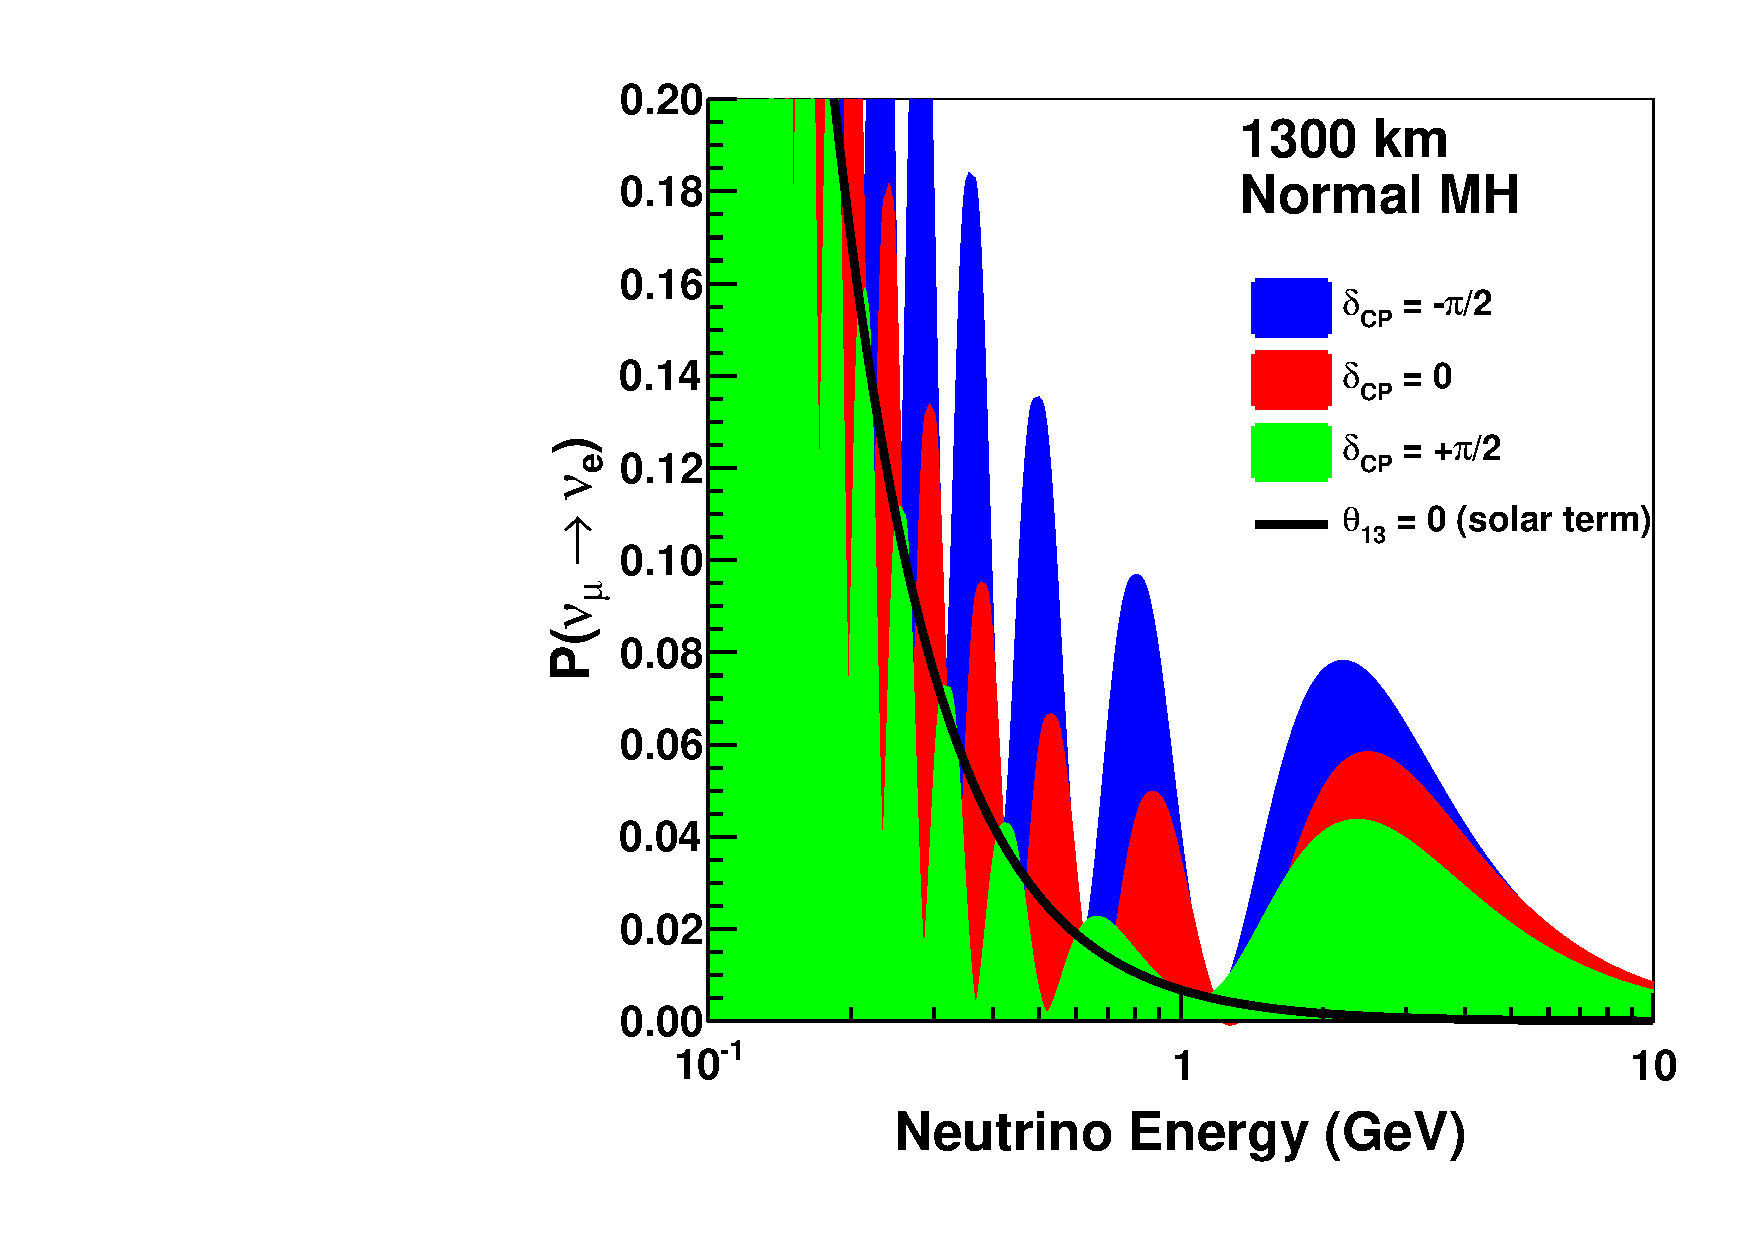
\includegraphics[width=0.45\linewidth]{energy_nu_no.pdf}
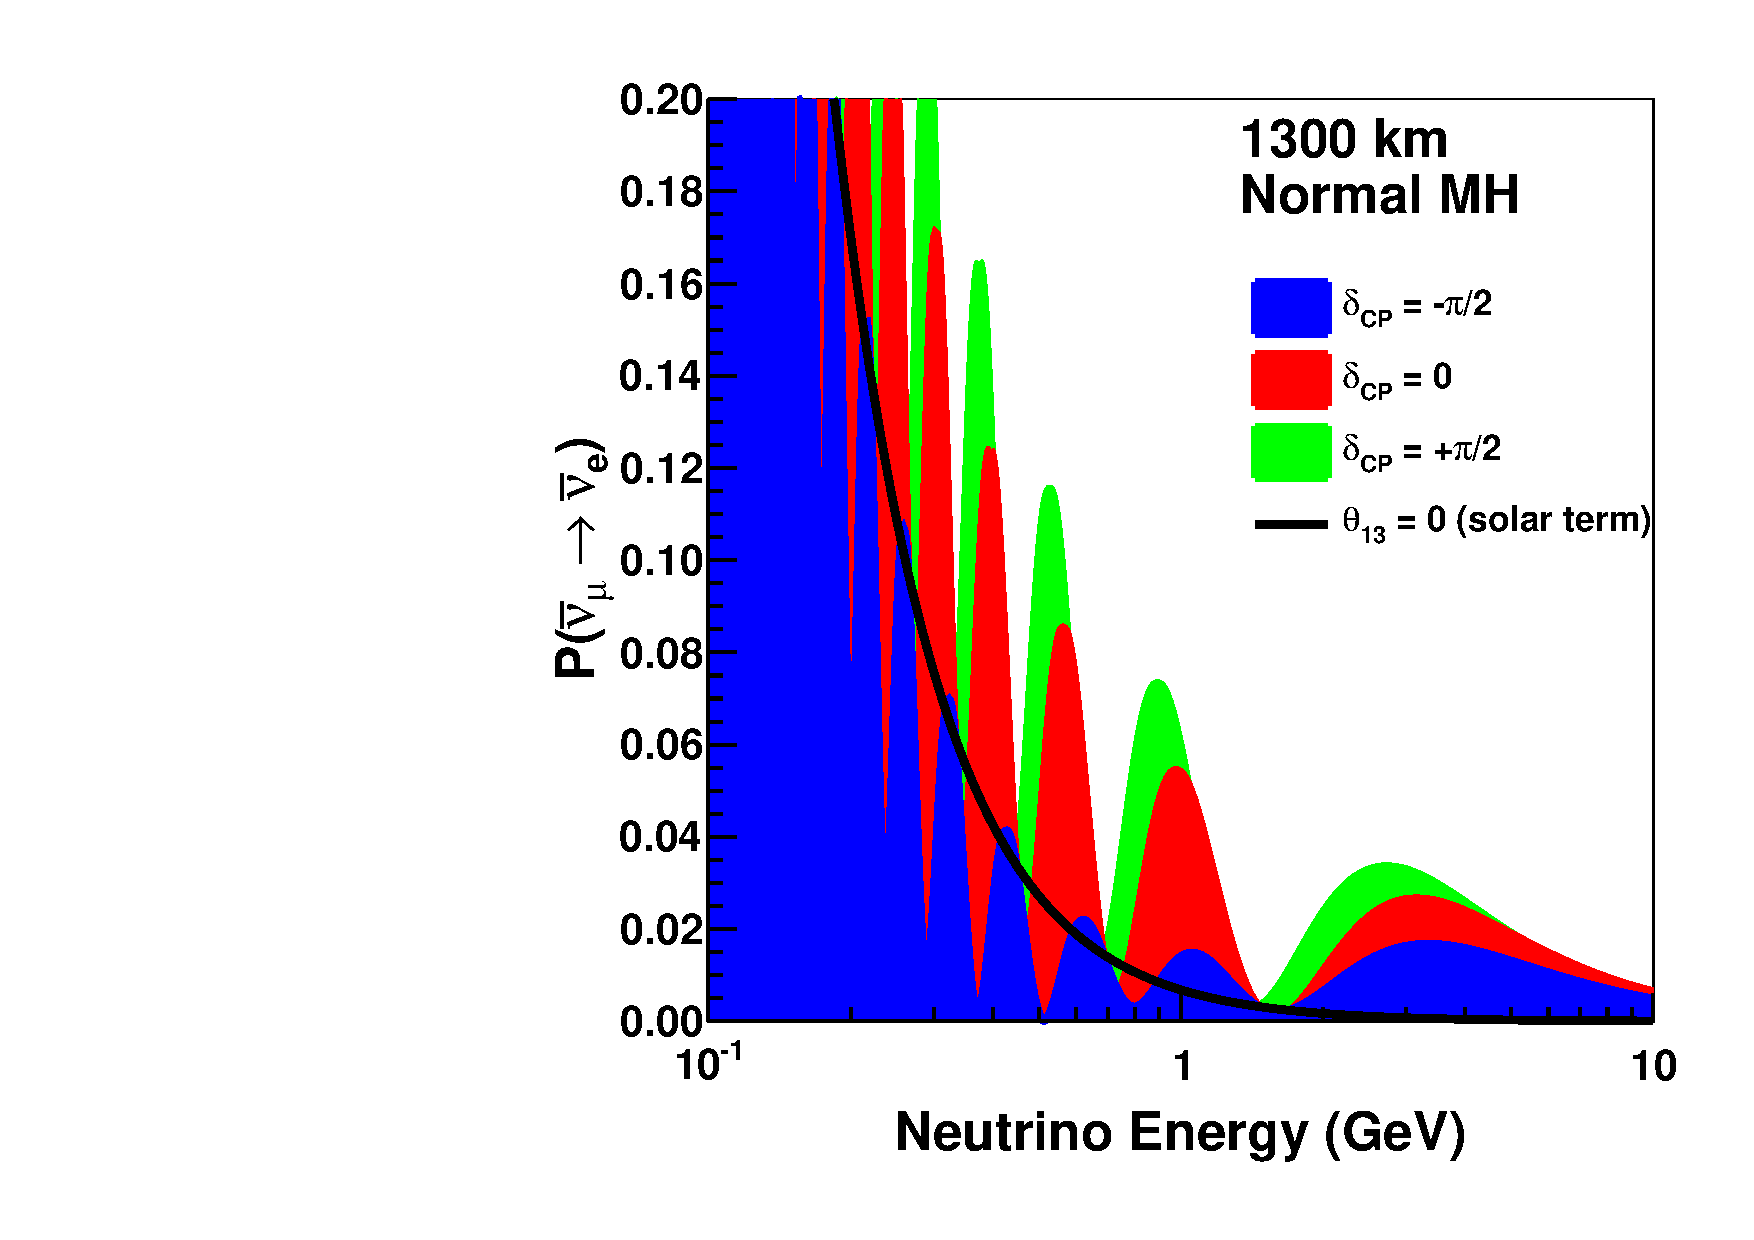
\includegraphics[width=0.45\linewidth]{energy_anu_no.pdf}
  \caption[Appearance probabilities for \nue and \anue at \SI{1300}{\km}]{The appearance probability at a baseline of \SI{1300}\km{},
  as a function of neutrino energy, for \deltacp = $-\pi/2$ (blue), 
  0 (red), and $\pi/2$ (green), for neutrinos (left) and antineutrinos
  (right), for normal ordering. The black line indicates the oscillation
  probability if $\theta_{13}$ were equal to zero. Note that DUNE will be built at a baseline of \SI{1300}{\km}}
  \label{fig:oscprob}
\end{figure}

In the particular expression of the PMNS matrix shown in
Equation~\ref{eqn:pmns}, the middle factor labeled ``II'' describes
the mixing between the $\nu_1$ and $\nu_3$ mass states, and depends on
the CP-violating phase \deltacp. The variation in the $\nu_\mu \rightarrow
\nu_e$ oscillation probability with the value of \deltacp
indicates that it is experimentally possible to measure the value of
\deltacp at a fixed baseline using only the observed shape of the
$\nu_\mu \rightarrow \nu_e$ {\em or} the 
$\bar{\nu}_\mu \rightarrow \bar{\nu}_e$
appearance signal measured over an energy range that encompasses at
least one full oscillation interval. A measurement of the value of
$\mdeltacp \neq 0 \ {\rm or} \ \pi$, assuming that neutrino mixing follows the three-flavor model, would imply \dword{cpv}. In the approximation for the electron neutrino appearance
probability given in Equation~\ref{eqn:appprob}, expanding the middle
term results in the presence of CP-odd terms (dependent on $\sin
\mdeltacp$) that have opposite signs in $\nu_{\mu} \rightarrow \nu_e$
and $\bar{\nu}_{\mu} \rightarrow \bar{\nu}_e$ oscillations.
For $\mdeltacp \neq 0$ or $\pi$, these terms introduce an asymmetry in
neutrino versus antineutrino oscillations. 
%This CP asymmetry, $\mathcal{A}_{CP}$, is defined as 
%\begin{equation}
%\label{eqn:cp-asymm}
% \mathcal{A}_{CP} = \frac{P(\nu_\mu \rightarrow \nu_e) -
%  P(\bar{\nu}_\mu \rightarrow \bar{\nu}_e)}{P(\nu_\mu \rightarrow
%  \nu_e) + P(\bar{\nu}_\mu \rightarrow \bar{\nu}_e)}.
%\end{equation}
%In the three-flavor model the asymmetry can be approximated to leading
%order in $\Delta m_{21}^2$ as~\cite{Marciano:2006uc}:
%\begin{equation}
%\mathcal{A}_{CP} \sim \frac{\cos \theta_{23} \sin 2 \theta_{12}
%  {\sin \mdeltacp}}{\sin \theta_{23} \sin \theta_{13}}
%\left(\frac{\Delta m^2_{21} L}{ 4 E_{\nu}}\right) + {\rm matter
%  \ effects}
%\label{eqn:cpasym}
%\end{equation}
Regardless of the measured value obtained for \deltacp, the explicit
%observation of the asymmetry $\mathcal{A}_{CP}$ in $\nu_{\mu}
observation of the asymmetry in $\nu_{\mu}
\rightarrow \nu_e$ and $\bar{\nu}_{\mu} \rightarrow
\bar{\nu}_e$ oscillations is sought to directly demonstrate the
leptonic \dword{cpv} effect.  
% A measurement of \deltacp that is inconsistent with the measurement of $\mathcal{A}_{CP}$ according toEquation~\ref{eqn:cpasym} could be evidence of physics beyond the standard three-flavor model.  
Furthermore, for long-baseline
experiments such as \dword{dune} where the neutrino beam propagates through
the Earth's mantle, the leptonic \dword{cpv} effects must be
disentangled from the matter effects.

The \SI{1300}{\km} baseline establishes one of \dword{dune}'s key strengths: sensitivity to the matter effect. This effect leads to a large asymmetry in the $\nu_\mu\to \nu_e$ versus $\bar{\nu}_\mu \to \bar{\nu}_e$ oscillation probabilities, the sign of which depends on the neutrino mass ordering.  At \SI{1300}{\km} this asymmetry is approximately $\pm 40\%$ in the region of the peak flux; this is larger than the maximal possible \dword{cp}-violating asymmetry associated with \deltacp, meaning that both the \dword{mh} and \deltacp can be determined
unambiguously with high confidence within the same experiment using the beam neutrinos. Concurrent analysis of the corresponding atmospheric-neutrino samples may provide an independent measurement of the neutrino mass ordering.

The rich oscillation structure that can be observed by \dword{dune} will enable precision measurement  in a single experiment of all the mixing parameters governing $\nu_1$-$\nu_3$ and $\nu_2$-$\nu_3$ mixing. Higher-precision measurements of the known oscillation parameters improves sensitivity to physics beyond the three-flavor oscillation model, particularly when compared to independent measurements by other experiments, including reactor measurements of $\theta_{13}$ and
measurements with atmospheric neutrinos. \dword{dune} will seek not only to demonstrate explicit \dword{cpv} by observing a difference in the neutrino and antineutrino oscillation probabilities, but also to precisely measure the value of \deltacp. 

% Theoretical models that consider quark-lepton universality predict specific values of the mixing angles and the relations between them. 
 The mixing angle $\theta_{13}$ has been measured accurately in reactor experiments. While the constraint on $\theta_{13}$ from the reactor experiments will be important in the
early stages of \dword{dune}, 
\dword{dune} itself will eventually be able to measure
$\theta_{13}$ independently with a similar precision to reactor experiments. 
Whereas the reactor experiments measure $\theta_{13}$ using $\bar{\nu}_e$ disappearance, \dword{dune} will measure it through $\nu_e$ and $\bar{\nu}_e$ appearance, thus providing an independent constraint on
the three-flavor mixing matrix.   

Current world measurements of \sinst{23} leave an ambiguity as to whether the value of $\theta_{23}$ is in the lower octant (less than 45\mbox{$^{\circ}$}), the upper octant (greater than 45\mbox{$^{\circ}$}), or exactly 45\mbox{$^{\circ}$}.  The value of $\sin^2 \theta_{23}$ from \dword{nufit}~\cite{Esteban:2018azc,nufitweb} is in the upper octant, but the distribution of the $\chi^{2}$ has another local minimum in the lower octant. A \emph{maximal} mixing value of $\sin^2 \theta_{23} =0.5$ is therefore still allowed by the data and the octant is still largely undetermined.  A value of
$\theta_{23}$ exactly equal to 45\mbox{$^{\circ}$} would indicate that $\nu_{\mu}$ and $\nu_{\tau}$ have equal contributions from $\nu_3$, which could be evidence for a previously unknown symmetry.  It is therefore important to experimentally determine the value of $\sin ^2
\theta_{23}$ with sufficient precision to determine the octant of $\theta_{23}$.

The magnitude of the
CP-violating terms in the oscillation depends most directly on the
size of the Jarlskog Invariant~\cite{Jarlskog:1985cw}, a function that
was introduced to provide a measure of CP violation independent of the
mixing-matrix parameterization. In terms of the parameterization
presented in Equation~\ref{eqn:pmns}, the Jarlskog Invariant is:
%
\begin{equation}
J_{CP}^{\rm PMNS} \equiv \frac{1}{8} \sin 2 \theta_{12} \sin 2 \theta_{13}
\sin 2 \theta_{23} \cos \theta_{13} \sin \mdeltacp.
\end{equation}
The relatively large values of the mixing angles in the lepton sector imply that
leptonic \dword{cpv} effects may be quite large, though this depends on
the value of \deltacp, which is currently unknown. Given the current best-fit values of the mixing angles~\cite{Esteban:2018azc,nufitweb} and assuming normal ordering,
\begin{equation}
J_{CP}^{\rm PMNS} \approx 0.03 \sin \mdeltacp.
\end{equation}
This is in sharp contrast to the very small mixing in the quark sector,  
which leads to a very small value of the corresponding quark-sector
Jarlskog Invariant~\cite{Tanabashi:2018oca}, %{Beringer:1900zz},
\begin{equation}
J_{CP}^{\rm CKM} \approx 3 \times 10^{-5},
\end{equation}
despite the large value of $\delta^{\rm CKM}_{CP}\approx70^{\circ}$.

A comparison among the values of the parameters in the neutrino
and quark sectors suggest that mixing in the two sectors may be
qualitatively different. Illustrating this difference, the value of
the entries of the \dword{ckm} %CKM 
quark-mixing matrix (analogous to the \dword{pmns} matrix for
neutrinos, and thus indicative of the strength of flavor-changing weak
decays in the quark sector) can be expressed in approximate form as
\begin{equation}
|V_{\rm CKM}|\sim \left(\begin{array}{ccc} 1 & 0.2 & 0.004\\ 0.2 & 1 & 0.04 \\ 0.008 & 0.04 & 1\end{array} \right),
\label{eq:ckmmatrix}
\end{equation}
for comparison to the entries of the \dword{pmns} matrix given in Equation~\ref{eq:pmnsmatrix}.
As discussed in \cite{King:2014nza}, the question of why the quark mixing angles are
smaller than the lepton mixing angles is an important part of the %``flavor problem.'' AH 5/9
flavor pattern question. Data on the patterns of neutrino mixing are already contributing to the quest to understand whether there is a relationship between quarks and leptons and their seemingly arbitrary generation structure.   

%ETW Nix this discussion as it irritates theorists
%To quote the discussion in~\cite{deGouvea:2013onf}, ``while the \dword{ckm}
%matrix is almost proportional to the identity matrix plus
%hierarchically ordered off-diagonal elements, the \dword{pmns} matrix is far
%from diagonal and, with the possible exception of the $U_{e3}$
%element, all elements are ${\cal O}(1)$.''
%A special role is played here by the fact that the magnitude of the smaller of the lepton mixing angles is similar to the larger of the quark mixing parameters, namely the Cabibbo angle~\cite{Boucenna:2012xb}.  Anne 3/9
%It is important here to note that the smaller of the lepton
%mixing angles is of similar magnitude to the larger of the quark mixing parameters, namely the \dword{cabangle}~\cite{Boucenna:2012xb}.
%One theoretical method often used to address this question involves the use of non-Abelian discrete
%subgroups of $SU(3)$ as flavor symmetries; the popularity of this method %comes partially 
%is due in part from
%the fact that these symmetries can give rise to the nearly \emph{tri-bi-maximal}\footnote{Tri-bi-maximal mixing refers to a form of the neutrino mixing matrix with effective bimaximal mixing of $\nu_\mu$ and $\nu_\tau$
%at the atmospheric scale ($L/E \sim$ \SI{500}{\km / \GeV}) and effective trimaximal
%mixing for $\nu_e$ with $\nu_\mu$ and $\nu_\tau$ 
%at the solar scale ($L/E \sim$ \SI{15000}{\km / %\GeV})~\cite{Harrison:2002er}.} 
%structure of the \dword{pmns} matrix.
%Whether employing these flavor symmetries or %other methods,
%any theoretical principle that attempts to %describe the fundamental
%symmetries implied by the observed organization of quark and neutrino
%mixing --- such as those proposed in unification models --- leads to
%testable predictions such as sum rules between \dword{ckm} and \dword{pmns}
%parameters~\cite{King:2014nza,deGouvea:2013onf,Mohapatra:2005wg,Albright:2006cw}.

%ETW Nix this discussion because it irritates me
%Clearly much work remains in order to complete the standard three-flavor 
%mixing picture, particularly 
%with regard to $\theta_{23}$ (is it less than, greater than, or equal
%to $45^\circ$?), mass ordering (normal or inverted?) 
%and \deltacp.
%Additionally, there is 
%great value in obtaining a set of measurements for multiple parameters 
%\emph{from a single experiment}, so that correlations and systematic 
%uncertainties can be handled properly.  Such an experiment will also be 
%well positioned to extensively test the standard picture of three-flavor mixing.  
%\dword{dune} is designed to be this experiment.

DUNE is designed to make significant contributions to completion of the standard three-flavor 
mixing picture. Scientific goals are definitive determination of the neutrino mass ordering, definitive observation of CP violation for more than 50\% of possible true \deltacp values,  
and precise measurement of oscillation parameters, particularly \deltacp, \sinstt{13}, and the octant of \sinst{23}. There is 
great value in obtaining this set of measurements in a single experiment using a broadband beam, so that the oscillation pattern may be clearly observed and a detailed test of the three-flavor neutrino model may be performed. 